\documentclass[border=1mm]{standalone}
% \usepackage[margin=2.5cm]{geometry}

\usepackage{graphicx,tikz,tikz-layers,amsmath,ifthen,tabularray} 
\usetikzlibrary{decorations.markings,calc,positioning,arrows,shapes.geometric,arrows.meta,matrix}

\colorlet{myred}{red!80!black}
\colorlet{myblue}{blue!80!black}
\colorlet{mybluee}{myblue!80!black}
\colorlet{mygreen}{green!60!black}
\colorlet{myorange}{orange!70!red!60!black}
\colorlet{mydarkred}{red!20!black}
\colorlet{mydarkblue}{blue!40!black}
\colorlet{mydarkgreen}{green!20!black}




\begin{document}

% \resizebox{\textwidth}{!}{
\tikz[font=\small, scale=1, every node/.style={outer sep=0pt, inner sep=0pt}, w/.style={minimum width=#1}, h/.style={minimum height=#1}, s/.style={minimum size=#1}, eu/.style={shorten >=#1}, ed/.style={shorten <=#1}, line join=round]
{
\tikzset{>={Latex[length=1.5mm, width=1.25mm]}}

\node[] (seagull) at (-4.5,.65) {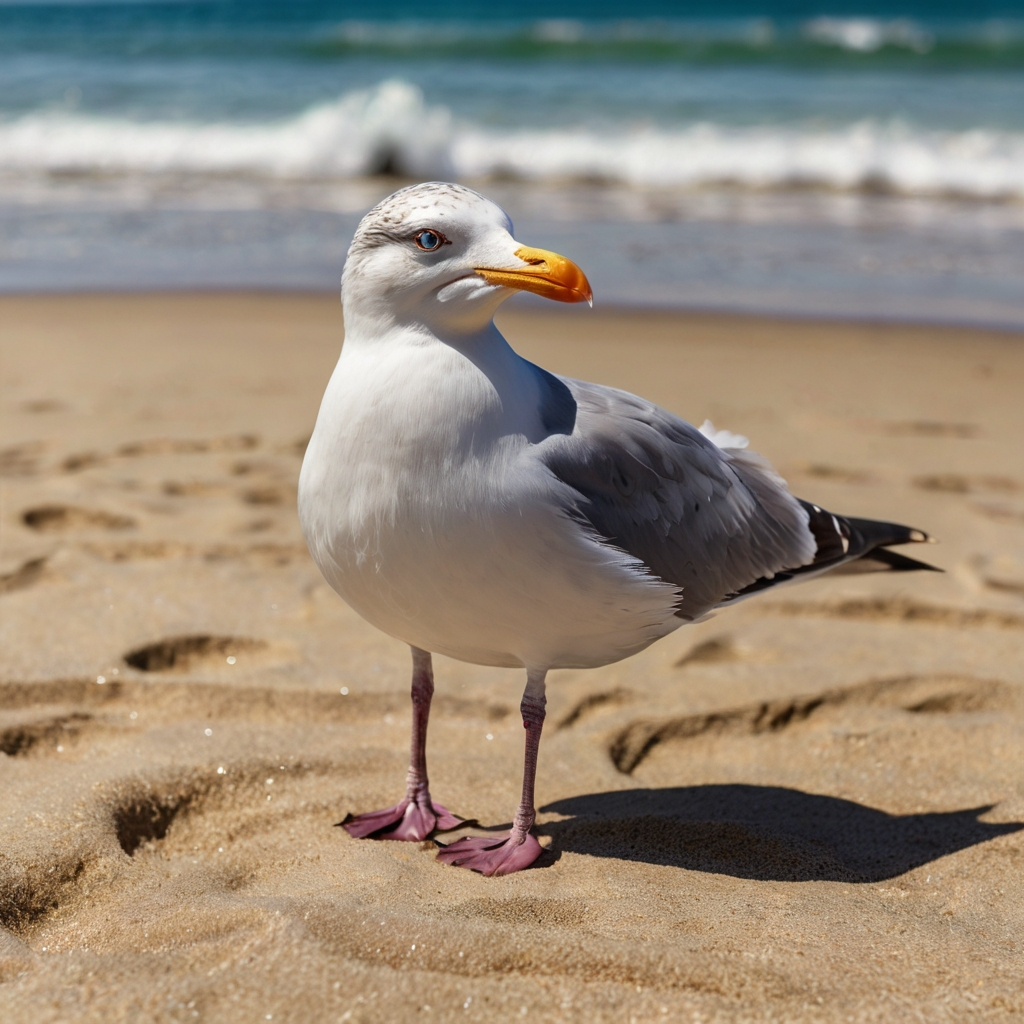
\includegraphics[width=3.1cm]{images/seagull.jpg}};

% Larger words
\node[text=myblue!60, font=\huge\bfseries] at (1,1) {gull};
\node[text=mydarkred!60, font=\Large\bfseries] at (-1.5,1.5) {beach};
\node[text=mybluee!60, font=\Large\bfseries] at (2.5,1.25) {bird};
\node[text=mygreen!60, font=\Large\bfseries] at (-1.5,-.5) {waves};

% Medium-sized words
\node[text=myorange!60, font=\large\bfseries] at (2,-.25) {subspecies};
\node[text=mydarkblue!60, font=\large\bfseries] at (-1.5,.5) {reintroduced};
\node[text=mydarkgreen!60, font=\large\bfseries] at (1,1.75) {version};
\node[text=myred!60, font=\large\bfseries] at (0,-.15) {ashore};

% Smaller words
\node[text=myblue!60, font=\normalsize\bfseries] at (-1,1) {photograph};
\node[text=mydarkred!60, font=\normalsize\bfseries] at (2,0.5) {wrecked};
\node[text=mygreen!60, font=\normalsize\bfseries] at (-2,0) {plumage};
\node[text=myorange!60, font=\normalsize\bfseries] at (0.5,0.25) {coasts};
\node[text=mydarkblue!60, font=\normalsize\bfseries] at (-0.5,2) {beaches};
\node[text=mybluee!60, font=\normalsize\bfseries] at (1.5,-.7) {schleswig};


\begin{scope}[xshift=10cm]
\node[] (cake) at (-4.5,.65) {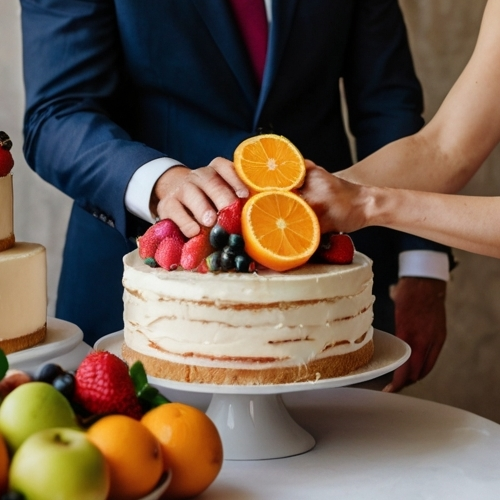
\includegraphics[width=3.1cm]{images/cake.jpg}};

% Larger words
\node[text=myblue!60, font=\huge\bfseries] at (1,.8) {cake};
\node[text=mydarkred!60, font=\huge\bfseries] at (2,1.5) {wedding};

% Medium-sized words
\node[text=mygreen!60, font=\Large\bfseries] at (-1.5,1) {weddings};
\node[text=mybluee!60, font=\Large\bfseries] at (-.5,2) {receptions};
\node[text=myorange!60, font=\Large\bfseries] at (-2,0.5) {tier};
\node[text=myred!60, font=\Large\bfseries] at (0.35,-.25) {traditionally};

% Smaller words
\node[text=mydarkblue!60, font=\normalsize\bfseries] at (1,0.25) {marriages};
\node[text=mygreen!60, font=\normalsize\bfseries] at (-.6,0.45) {fruits};
\node[text=myblue!60, font=\normalsize\bfseries] at (-0.5,1.5) {cheese};
\node[text=mydarkred!60, font=\normalsize\bfseries] at (2.5,1) {slicing};
\node[text=myorange!60, font=\normalsize\bfseries] at (2.7,0) {grapes};
\node[text=mybluee!60, font=\normalsize\bfseries] at (-2,0) {berries};
\node[text=myred!60, font=\normalsize\bfseries] at (2.6,.5) {lighted};
\node[text=mydarkgreen!60, font=\normalsize\bfseries] at (-1.5,-.7) {parties};
\end{scope}

\node[draw, densely dashed, w=6.2cm, h=3.07cm, anchor=west] at (seagull.east) {};
\node[draw, densely dashed, w=6.5cm, h=3.07cm, anchor=west] at (cake.east) {};



}

% }



\end{document}
